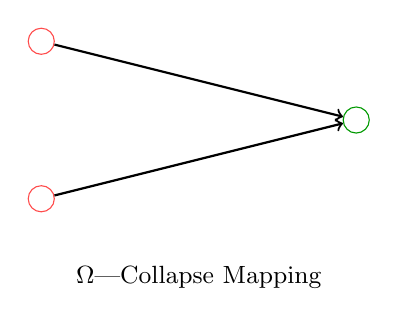
\begin{tikzpicture}[
    old/.style={circle,draw=red!70,fill=white,minimum size=5pt},
    new/.style={circle,draw=green!60!black,fill=white,minimum size=6pt},
    arrow/.style={->, thick}
]

\node[old] (O1) at (-2,1) {};
\node[old] (O2) at (-2,-1) {};

\node[new] (N1) at (2,0) {};

\draw[arrow] (O1)--(N1);
\draw[arrow] (O2)--(N1);

\node at (0,-2) {\small $\Omega$---Collapse Mapping};

\end{tikzpicture}